% Options for packages loaded elsewhere
\PassOptionsToPackage{unicode}{hyperref}
\PassOptionsToPackage{hyphens}{url}
%
\documentclass[
]{article}
\usepackage{lmodern}
\usepackage{amssymb,amsmath}
\usepackage{ifxetex,ifluatex}
\ifnum 0\ifxetex 1\fi\ifluatex 1\fi=0 % if pdftex
  \usepackage[T1]{fontenc}
  \usepackage[utf8]{inputenc}
  \usepackage{textcomp} % provide euro and other symbols
\else % if luatex or xetex
  \usepackage{unicode-math}
  \defaultfontfeatures{Scale=MatchLowercase}
  \defaultfontfeatures[\rmfamily]{Ligatures=TeX,Scale=1}
\fi
% Use upquote if available, for straight quotes in verbatim environments
\IfFileExists{upquote.sty}{\usepackage{upquote}}{}
\IfFileExists{microtype.sty}{% use microtype if available
  \usepackage[]{microtype}
  \UseMicrotypeSet[protrusion]{basicmath} % disable protrusion for tt fonts
}{}
\makeatletter
\@ifundefined{KOMAClassName}{% if non-KOMA class
  \IfFileExists{parskip.sty}{%
    \usepackage{parskip}
  }{% else
    \setlength{\parindent}{0pt}
    \setlength{\parskip}{6pt plus 2pt minus 1pt}}
}{% if KOMA class
  \KOMAoptions{parskip=half}}
\makeatother
\usepackage{xcolor}
\IfFileExists{xurl.sty}{\usepackage{xurl}}{} % add URL line breaks if available
\IfFileExists{bookmark.sty}{\usepackage{bookmark}}{\usepackage{hyperref}}
\hypersetup{
  pdftitle={Report},
  pdfauthor={YOUR NAME HERE},
  hidelinks,
  pdfcreator={LaTeX via pandoc}}
\urlstyle{same} % disable monospaced font for URLs
\usepackage[margin=1in]{geometry}
\usepackage{color}
\usepackage{fancyvrb}
\newcommand{\VerbBar}{|}
\newcommand{\VERB}{\Verb[commandchars=\\\{\}]}
\DefineVerbatimEnvironment{Highlighting}{Verbatim}{commandchars=\\\{\}}
% Add ',fontsize=\small' for more characters per line
\usepackage{framed}
\definecolor{shadecolor}{RGB}{248,248,248}
\newenvironment{Shaded}{\begin{snugshade}}{\end{snugshade}}
\newcommand{\AlertTok}[1]{\textcolor[rgb]{0.94,0.16,0.16}{#1}}
\newcommand{\AnnotationTok}[1]{\textcolor[rgb]{0.56,0.35,0.01}{\textbf{\textit{#1}}}}
\newcommand{\AttributeTok}[1]{\textcolor[rgb]{0.77,0.63,0.00}{#1}}
\newcommand{\BaseNTok}[1]{\textcolor[rgb]{0.00,0.00,0.81}{#1}}
\newcommand{\BuiltInTok}[1]{#1}
\newcommand{\CharTok}[1]{\textcolor[rgb]{0.31,0.60,0.02}{#1}}
\newcommand{\CommentTok}[1]{\textcolor[rgb]{0.56,0.35,0.01}{\textit{#1}}}
\newcommand{\CommentVarTok}[1]{\textcolor[rgb]{0.56,0.35,0.01}{\textbf{\textit{#1}}}}
\newcommand{\ConstantTok}[1]{\textcolor[rgb]{0.00,0.00,0.00}{#1}}
\newcommand{\ControlFlowTok}[1]{\textcolor[rgb]{0.13,0.29,0.53}{\textbf{#1}}}
\newcommand{\DataTypeTok}[1]{\textcolor[rgb]{0.13,0.29,0.53}{#1}}
\newcommand{\DecValTok}[1]{\textcolor[rgb]{0.00,0.00,0.81}{#1}}
\newcommand{\DocumentationTok}[1]{\textcolor[rgb]{0.56,0.35,0.01}{\textbf{\textit{#1}}}}
\newcommand{\ErrorTok}[1]{\textcolor[rgb]{0.64,0.00,0.00}{\textbf{#1}}}
\newcommand{\ExtensionTok}[1]{#1}
\newcommand{\FloatTok}[1]{\textcolor[rgb]{0.00,0.00,0.81}{#1}}
\newcommand{\FunctionTok}[1]{\textcolor[rgb]{0.00,0.00,0.00}{#1}}
\newcommand{\ImportTok}[1]{#1}
\newcommand{\InformationTok}[1]{\textcolor[rgb]{0.56,0.35,0.01}{\textbf{\textit{#1}}}}
\newcommand{\KeywordTok}[1]{\textcolor[rgb]{0.13,0.29,0.53}{\textbf{#1}}}
\newcommand{\NormalTok}[1]{#1}
\newcommand{\OperatorTok}[1]{\textcolor[rgb]{0.81,0.36,0.00}{\textbf{#1}}}
\newcommand{\OtherTok}[1]{\textcolor[rgb]{0.56,0.35,0.01}{#1}}
\newcommand{\PreprocessorTok}[1]{\textcolor[rgb]{0.56,0.35,0.01}{\textit{#1}}}
\newcommand{\RegionMarkerTok}[1]{#1}
\newcommand{\SpecialCharTok}[1]{\textcolor[rgb]{0.00,0.00,0.00}{#1}}
\newcommand{\SpecialStringTok}[1]{\textcolor[rgb]{0.31,0.60,0.02}{#1}}
\newcommand{\StringTok}[1]{\textcolor[rgb]{0.31,0.60,0.02}{#1}}
\newcommand{\VariableTok}[1]{\textcolor[rgb]{0.00,0.00,0.00}{#1}}
\newcommand{\VerbatimStringTok}[1]{\textcolor[rgb]{0.31,0.60,0.02}{#1}}
\newcommand{\WarningTok}[1]{\textcolor[rgb]{0.56,0.35,0.01}{\textbf{\textit{#1}}}}
\usepackage{longtable,booktabs}
% Correct order of tables after \paragraph or \subparagraph
\usepackage{etoolbox}
\makeatletter
\patchcmd\longtable{\par}{\if@noskipsec\mbox{}\fi\par}{}{}
\makeatother
% Allow footnotes in longtable head/foot
\IfFileExists{footnotehyper.sty}{\usepackage{footnotehyper}}{\usepackage{footnote}}
\makesavenoteenv{longtable}
\usepackage{graphicx,grffile}
\makeatletter
\def\maxwidth{\ifdim\Gin@nat@width>\linewidth\linewidth\else\Gin@nat@width\fi}
\def\maxheight{\ifdim\Gin@nat@height>\textheight\textheight\else\Gin@nat@height\fi}
\makeatother
% Scale images if necessary, so that they will not overflow the page
% margins by default, and it is still possible to overwrite the defaults
% using explicit options in \includegraphics[width, height, ...]{}
\setkeys{Gin}{width=\maxwidth,height=\maxheight,keepaspectratio}
% Set default figure placement to htbp
\makeatletter
\def\fps@figure{htbp}
\makeatother
\setlength{\emergencystretch}{3em} % prevent overfull lines
\providecommand{\tightlist}{%
  \setlength{\itemsep}{0pt}\setlength{\parskip}{0pt}}
\setcounter{secnumdepth}{5}
\usepackage{booktabs}
\usepackage{subfig}

\title{Report}
\author{YOUR NAME HERE}
\date{August 17, 2020}

\begin{document}
\maketitle

Note you will need \texttt{bookdown} package installed to render this template. It allows easy cross-referencing figures and tables. See \href{https://bookdown.org/yihui/rmarkdown-cookbook/cross-ref.html}{here}.

\hypertarget{description}{%
\section{Description}\label{description}}

Add your project description here.

You may choose to include an image from your experiment to describe your experiment. Please keep your image file in the same directory as your Rmd file so that you don't need to list the full path to your file. This helps the grading TA to run your Rmd file without worrying about incorrect file paths. Your can refer to Figure \ref{fig:speedgun} with \texttt{Figure\ \textbackslash{}@ref(fig:speedgun)}.

\begin{figure}

{\centering 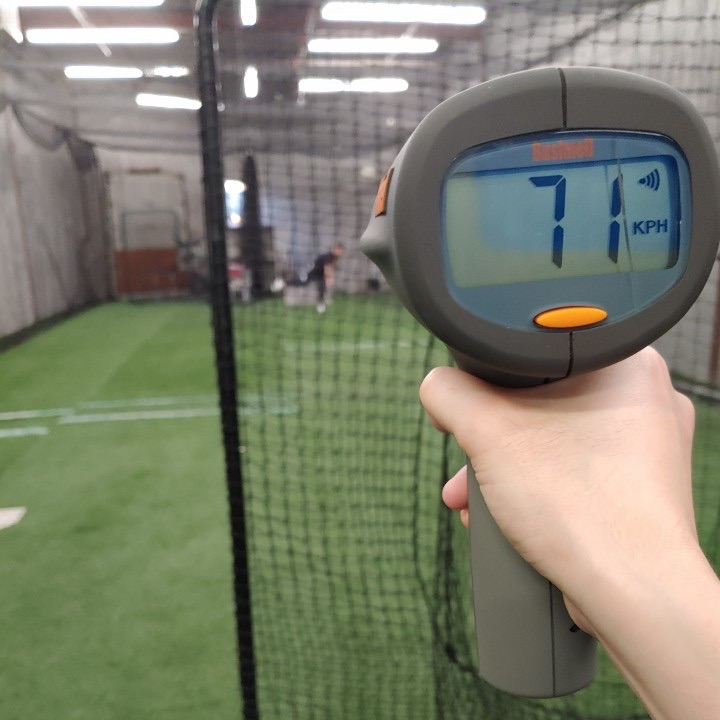
\includegraphics[width=.3\linewidth]{measure} 

}

\caption{Remeber to include an appropriate caption for your figures.}\label{fig:speedgun}
\end{figure}

\hypertarget{analysis}{%
\section{Analysis}\label{analysis}}

Add your analysis method and results here.

Below is a sample code for reading a data file for your project. Alternatively, you may choose to input your outcomes directly in R, but this is not recommended as it is more difficult to catch typos.

\begin{Shaded}
\begin{Highlighting}[]
\CommentTok{# If you plan to use a separate data file,}
\CommentTok{# I recommend using a csv format. A spreadsheet}
\CommentTok{# software (e.g., MS Excel, Apple Numbers) provide}
\CommentTok{# options to export your tables in the csv format.}
\CommentTok{# Keep your csv file in the same directory as your}
\CommentTok{# Rmd file so that you don't need to list the full}
\CommentTok{# path to your file. This helps the grading TA}
\CommentTok{# to run your Rmd file without worrying about}
\CommentTok{# incorrect file paths.}
\NormalTok{results <-}\StringTok{ }\KeywordTok{read.csv}\NormalTok{(}\StringTok{'data.csv'}\NormalTok{)}
\end{Highlighting}
\end{Shaded}

Table \ref{tab:tab1} is a sample table. It is not recommended that you include of a table to show the whole data but you may want to include tables for summary statistics and other analysis results. You can refer to the table using \texttt{Table\ \textbackslash{}@ref(tab:tab1)}.

\begin{table}

\caption{\label{tab:tab1}Your caption for tables go here.}
\centering
\begin{tabular}[t]{rllr}
\toprule
X & leg.kick & finger.split & observed.speed\\
\midrule
17 & N & Y & 87\\
19 & N & Y & 82\\
9 & Y & Y & 86\\
7 & Y & Y & 83\\
5 & Y & Y & 84\\
\addlinespace
15 & N & Y & 87\\
6 & Y & N & 86\\
3 & Y & Y & 85\\
18 & N & N & 85\\
10 & Y & N & 86\\
\addlinespace
20 & N & N & 85\\
4 & Y & N & 87\\
14 & N & N & 83\\
11 & N & Y & 86\\
16 & N & N & 87\\
\addlinespace
1 & Y & Y & 84\\
2 & Y & N & 84\\
13 & N & Y & 88\\
12 & N & N & 90\\
8 & Y & N & 85\\
\bottomrule
\end{tabular}
\end{table}

Figure \ref{fig:fig2} is a sample for placing subfigures in your report. Feel free to reuse the code to place your own plots. You will need to generate the appropriate plots that fit your own experiment.

\begin{figure}

{\centering \subfloat[This is caption for the first subfigure.\label{fig:fig2-1}]{\includegraphics[width=.4\linewidth]{report_files/figure-latex/fig2-1} }\subfloat[This is caption for the second figure\label{fig:fig2-2}]{\includegraphics[width=.4\linewidth]{report_files/figure-latex/fig2-2} }

}

\caption{This is figure caption for all subfigures.}\label{fig:fig2}
\end{figure}

\hypertarget{conclusions-and-discussions}{%
\section{Conclusions and Discussions}\label{conclusions-and-discussions}}

Add your conclusions and any additional discussions here.

\end{document}
